\chapter{Statistics in Cosmology} % Main chapter title

\label{Statis} % For referencing the chapter elsewhere, use \ref{Chapter1} 

%----------------------------------------------------------------------------------------

\section{The relation between Gaussianity, linearity and homogeneity}

\subsection{Gaussian random fields}

In cosmology, we are interested in studying obervables which have been the product of a large number of random processes.
The best examples are the fluctuations of temperature in the CMB $\delta T / T$ or the fluctuations of the matter density in the Universe, 
usually called $\delta$, which originate from complicated interactions between different matter species, gravity and other fundamental forces.
Using the Central Limit Theorem \cite{(cite...)}, we can show that the sum of a large number of random variables, that originate from independent random processes, will yield a variable that it is almost exactly Gaussian distributed. The Gaussian probability distribution $p(x)$ for a random variable $x$, with mean $\mu$ and variance $\sigma$ is given by
\begin{equation}
p(x) = \frac{1}{\sqrt{2 \pi \sigma^2}}\exp\left( \frac{(x-\mu)^2}{2\sigma^2} \right)
\end{equation}
As we sill see, Gaussianly distributed variables will be very important in observations and analysis of cosmological observables.
In the case of structure formation, $\delta$ is a random field that describes inhomogeneities, however, due to the 
assumption that it originates from independent random processes in a homogeneous and isotropic universe,
its statistical properties must be homogeneous and isotropic too \cite{(cite...Peacock, Bjoern, ?)}.
That means that the probability distribution $p(\delta(\vec{x}))$ must be invariant under translations and rotations of space.
The expectation value of $\langle \delta^n \rangle$ is formally speaking defined by an ensemble average, meaning that
we should actually observe this process in many random realizations of the Universe. Since this is not possible,
in cosmology we postulate the ergodicity principle \cite{(cite Adler...)}, which states that for sufficient large volumes
the ensemble average is equal to the volume average and therefore, we can write:
\begin{equation}
\langle \delta^n \rangle = \frac{1}{V} \int_V \mathrm{d}^3 x \, \delta^n (\vec{x}) p(\delta (\vec{x}))
\end{equation} 
The importance of this postulate in practical terms is that we can use our formal statistical tools 
to compute theoretically the expectation values
of observables and in the observational side, we just need to match this by observing over large volumes in the sky.

\subsection{The two-point correlation function}

The advantage of working with fluctuation variables in cosmology is that their mean is zero, i.e. $\langle \delta \rangle = 0$
and that they remain small ($\delta<<1$) for most of their evolution time.
Therefore what makes sense to study is not its mean, but its variance, $\langle \delta^2 \rangle$, or if 
we are measuring the fluctuations at two separated points in the universe ($\vec{x}$ and $\vec{y}$),
then it makes sense to study their two-point correlation function, defined as:
\begin{equation} \label{eq:correlationfunct}
\xi(\vec{x} ,\vec{y}) = \langle \delta (\vec{x})  \delta (\vec{y}) \rangle
\end{equation}
As we have seen before, $\delta$ is statistically homogeneous and isotropic. Therefore, due to homogeneity, the correlation
function can only depend on separation $\vec r = \vec{x}_2 - \vec{x}_1 $ and due to invariance under 
rotations it can only depend on the magnitude of the separation, denoted as $r$.
In simple words---for the case of large scale structure---, $\xi(r)$ is telling us how probable it is to find
a galaxy a distance $r$ away from a given galaxy at position $\vec x$.
We are talking here about ideal measurements for a linear and Gaussian observable, but in the later chapters, when we discuss
about non-linearities and observational effects (for example redshift space distortions), we will see that the situation is in practice not so simple and 
the observable $\delta$, will not be specified only by its 
two-point correlation function and will not be statistically isotropic, leading to different correlation
functions parallel and perpendicular to the line of sight \cite{(cite some BAO stuff)}.

\subsection{The data covariance matrix}

Let us introduce at this point the \emph{data} covariance matrix, since this is a concept that causes a lot of misunderstanding in the literature,
when it is confused with the \emph{parameter} covariance matrix, which will be introduced later.
If we are measuring the fluctuation $\delta$ at three points in space,  $\vec{x}, \vec{y}$ and $\vec{z}$,
then their joint probability density will still be Gaussian:
\begin{equation}\label{eq:multivariateGaussian}
p( \delta (\vec{x}),\delta (\vec{y}),\delta (\vec{z})) = 
\frac{1}{\sqrt{(2 \pi)^2 \det \mathbf{C}}}\exp\left( -\frac{1}{2} \colvec{3}{\delta(\vec{x})}{\delta(\vec{y})}{\delta(\vec{z})}^T 
\mathbf{C}^{-1} \colvec{3}{\delta(\vec{x})}{\delta(\vec{y})}{\delta(\vec{z})}
 \right)
\end{equation}
where now instead of a Gaussian dispersion $\sigma$, we have a Gaussian \emph{data} covariance matrix $\mathbf{C}$, given by:
\begin{equation}\label{eq:dataCovariance-abstract}
C_ij = 
\begin{pmatrix}
\langle \delta^2 (\vec{x}) \rangle 
                & \langle \delta (\vec{x}) \delta (\vec{y})\rangle 
                        & \langle \delta (\vec{x})  \delta (\vec{z})\rangle  \\
\langle \delta (\vec{x})  \delta (\vec{y})\rangle 
                & \langle \delta^2 (\vec{y}) \rangle 
                        & \langle \delta (\vec{y})  \delta (\vec{z})\rangle  \\
\langle \delta (\vec{x})  \delta (\vec{z})\rangle 
                & \langle \delta (\vec{y}) \delta (\vec{z})\rangle 
                        & \langle \delta^2 (\vec{z})  \rangle  \\
\end{pmatrix}
\end{equation}
Notice that the covariance matrix is symmetric and positive definite. This is the data covariance matrix for three measurements
in real space. If you would measure the density fluctuations at 1000 different points in space, the covariance matrix would 
have 1 million elements. Therefore, it is very important not only for theoretical, but for practical reasons of data analysis, that the covariance matrix is as simple and symmetric as possible.

Luckily, for Gaussian random fields their statistical properties can be defined entirely by the their two-point correlation function,
where the following recursion relations (obtained by Isserli's or Wick's theorem \cite{(cite Wick or something)}) are valid:
\begin{align}
\langle \delta^{2n}\rangle = (2n-1)!!\langle \delta \rangle \, & ,\quad \langle \delta^{2n+1}\rangle =0
\end{align}
This is of course expected, 
since we have defined in Eqn. \ref{eq:multivariateGaussian} the covariance matrix $\mathbf{C}$ as the only statistical quantity needed to specify
fully the distribution of the multivariate  Gaussian random field.

\subsection{The power spectrum}

Since we want observations of $\delta$ to be independent of each other, we need that the equations governing the spatial 
distribution of the density fluctuations are linear, otherwise non-linear terms can induce correlations between 
values at different positions. We can see this more clearly if we work in Fourier space.
For linear equations, transforming into Fourier space (going from position $\vec x$ to wavevectors $\vec k$) is quite useful, 
since space derivatives become simply factors of $\vec k$ and the Fourier space function $\delta(\vec k)$
evolves in time, independently for each $k$-mode, but only if the field is statistically homogeneous.

The Fourier transform of the density field, denoted $\delta(\vec k)$ is defined as:
\begin{equation}
\delta(\vec k) = \int \mathrm{d}^3 x \delta(\vec x) \exp(-i \vec{k} \cdot \vec{x})
\end{equation}
and its inverse is
\begin{equation}
\delta(\vec x) = \int \frac{\mathrm{d}^3 k}{(2\pi^3)} \delta(\vec k) \exp(i \vec{k} \cdot \vec{x}) \quad .
\end{equation}
Since now $\delta(\vec k)$ can be complex, we can define the variance between two $k$-modes as:
\begin{equation}
\langle \delta (\vec{k}_1)  \delta^{*} (\vec{k}_2) \rangle = 
\int \mathrm{d}^3 x \, \mathrm{d}^3 y \langle \delta (\vec{x})  \delta (\vec{y}) \rangle \exp(-i \vec{k} \cdot (\vec{x}-\vec{y}) )
(2\pi)^3 \delta_{D}(\vec{k}_{1}-\vec{k}_{2})  \quad .
\end{equation}
Using the definition of the correlation function \ref{eq:correlationfunct} and the fact that the Gaussian random field $\delta$
is homogeneous we can define the power spectrum $P(\vec k)$ as:
\begin{equation}\label{eq:powerspectrum}
P(\vec k) = \int \mathrm{d}^3r \, \xi(\vec r) \exp(-i \vec{k} \cdot \vec{r})
\end{equation}
The relation between the expected value of $\langle \delta (\vec{k}_1)  \delta^{*} (\vec{k}_2) \rangle$ and the power spectrum $P(\vec k)$ can be obtained by a similar straightforward calculation, \cite{(cite Luca, Dodelson, ??)} where taking into account
that the $\delta$ field is real-valued, one can obtain:
\begin{equation}
\langle \delta (\vec{k}_1)  \delta (\vec{k}_2) \rangle = (2\pi)^3  P(k) \delta_{D}(\vec{k}_{1}-\vec{k}_{2}) \quad .
\end{equation}
The Dirac delta $\delta_D$ in the previous equation, shows us directly what we had expected from a random Gaussian and homogeneous field;
the Fourier modes $\vec{k}_1$ and $\vec{k}_2$ for the density fluctuations are mutually uncorrelated.
In this case, the data covariance matrix $\mathbf{C}$, defined in Eqn. \ref{eq:dataCovariance-abstract},
would be perfectly diagonal in Fourier space, making an analysis of the observations much more tractable.

However, this is only true if the equations governing $\delta$ are linear; otherwise, non-linear terms in real space,
would introduce convolutions in Fourier space, giving rise to non-vanishing correlations $\langle \delta (\vec{k}_1)  \delta (\vec{k}_2) \rangle$. This will be the subject of study of the non-linear power spectrum, which will be treated with more depth in chapter \ref{chap:nonlinear}.

\subsection{Final remarks on linearity, Gaussianity and homogeneity}

We have seen in the previous sections, that the concepts of linearity, Gaussianity and homogeneity
are strongly related in Cosmology.
The fact that observables like the matter density fluctuations originate from a large number 
of independent random processes, leads---thanks to the Central Limit Theorem---to a Gaussian random field.
Then homogeneity and isotropy of the Universe and linear equations (in space) governing those processes, ensure that the statistical properties of the Gaussian random field
are also homogeneous and isotropic and that we can use the ergodic theorem to compute ensemble averages.
The Gaussianity of the field (and its vanishing average value) allows us to describe the field, solely with its two
point correlation function, which directly connects us to the power spectrum and then to the fact that in Fourier space, 
pairs of wavemodes are mutually uncorrelated.
\begin{equation}
\textrm{Gaussianity}\Leftrightarrow\textrm{Linearity}\Leftrightarrow\textrm{Homogeneity}
\end{equation}

In contrast, non-linear evolution of the density field, would yield correlations among different $k$-modes, 
leading to a non-Gaussian probability distribution and the loss of homogeneity (or the appearance of $k$-dependent growth).
This is exactly what happens at later stages of structure formation, 
where fluctuations are limited to $-1 < \delta$ in voids, 
but can grow to very high values $\delta \gg 1$ inside the cosmic web structure.
This in turn will make the data covariance matrix $\mathbf{C}$ in Fourier space not diagonal anymore and 
will difficult the analysis of cosmological observations.
Therefore, the computation
of these non-linear evolution equations 
and the analysis of higher order correlations is one of the great challenges that research in cosmology 
will have to face in the next decade.


\section{Likelihood and the Bayesian approach}

The subject of Bayesian statistics is a very complex, but very important topic in modern
statistics, data science and the physical sciences \cite{cite Gregory and others}
and it is outside of the scope of this work to try to even review its more fundamental properties.
We will just comment on the simple but very powerful concept of the likelihood function and how the Bayesian
approach to statistical analysis is best suited in a field like cosmology.

If an experiment yields a vector of random variables $x^i$, 
we have to
try to build a theoretical model, which depends on some free parameters $\theta^i$ 
that can give us the probability distribution $p(x^i | \theta^i)$ to find the variable $x^i$ 
inside an interval $\Delta x$ for a specific measurement.
Then what physicists are interested in, is in constraining the model parameters $\theta$ and try to find
the set of parameters (or the model) that best explains the data.

There are two possibilities of analyzing the results of that experiment, the \emph{frequentist}
and the \emph{Bayesian} approach.

In the \emph{frequentist} approach, the scientist would repeat many times the experiment and even change
the settings and the theoretical parameters $\theta$ in the lab, in order to find the distribution
of $x^i$'s ($p(x^i | \theta^i)$) and from there, infer the distribution of the parameters $\theta$. So this scientist would
be able to say (as it is usually done in particle physics) that a there is a 97\% probability that her 
data is distributed according to the model she has found as best fit (where one parameter is for example the Higgs mass).

In the \emph{Bayesian} approach, the reasoning is reversed. The scientist would look for the probability
of having a certain model (with model parameters) given the data that has already been taken ($p(\theta^i | x^i)$). This is more suitable
for cosmology, since we cannot repeat many times the same experiment and we cannot change
the parameters of the Universe.

How do we then "invert" $P(D | T)$ ---the probability of the data given a model--- to obtain $P(T | D)$? The solution is given by 
Bayes' theorem \cite{Bayes, Dodelson, Luca, many}:

\beeq$ \label{eq:BayesTheorem}
P(T | D) = \frac{P(D | T) P(T)}{P(D)}$
$P(T | D)$ is usually called the posterior probability (of having a theory $T$ given the data $D$), 
$P(T)$ is the prior probability on the theory (which quantifies our previous knowledge and prejudices)
and $P(D)$ is the evidence (the probability of the data), which for all purposes we can ignore, since it
represents just a normalization factor.
Also here, a discussion on the significance and the effects of the prior is out of our scope. \cite{cite Amendola, Dodelson, Gregory, reviews}. However, in our case it will be an efficient way of combining results from previous
experiments into our predictions for future experiments. The prior can be as simple as the theoretical expectation
that a parameter cannot be zero (for example the matter density of the Universe) or it can be the entire
probability distribution of a previous experiment.
After this point we will roughly call the posterior $P(T | D)$ by its more common name: the likelihood function
$L(\theta | x)$.

From the likelihood we can obtain some useful quantities:
\begin{itemize}
	\item The maximum likelihood estimators $\hat{\theta}_{i}$,
	which are found by solving \\ $\partial L(\theta_i)/\partial\theta_i = 0$.
	This would amount to the 'best fit' parameters, but they
	are in general different tp the frequentist ones, if we have used a prior.
	\item The confidence regions for the parameters, denoted $R(\alpha)$, for which
	the normalized likelihood integrated in that region has a specific value:\\ $\int_{R(\alpha)}  L(\theta_i) \mathrm{d}^n \theta = \alpha$.
	If $\alpha=0.683,0.954,0.997$, this regions are called 1, 2 and 3$\sigma$ regions respectively.
	\item Marginalization over a parameter. If the likelihood depends on 
	three parameters $\theta^1, \theta^2, \theta^3$, but we are not interested in $\theta^3$, because it is a nuisance parameter
	or we have no clear idea how to relate it to the theory, we can marginalize over it by integrating 
	it out: $L(\theta_1, \theta_2) = \int L(\theta^1, \theta^2, \theta^3) \,\mathrm{d}\theta^3 $
	
\end{itemize}

Despite the great usefulness of the likelihood, its evaluation represents a challenge both numerically
and computationally, since it is a complicated multi-
dimensional function.
Evaluating the likelihood for a relatively coarse grid of points in parameter space, becomes unfeasible for 
more than 7 or 8 parameters. So, techniques like Markov Chain Monte Carlo (MCMC) \cite{cite some basic MCMC literature}
 have become more and more sophisticated. In this techniques, the basic idea is to explore the parameter
 space using a random walk, which is itself guided by the steepness or flatness of the likelihood at that point.
 In this way there are much less evaluations in places where the likelihood is smooth and many evaluations
 where the likelihood changes very rapidly. Two very well known
 codes in the cosmological community are \textsc{MontePython} and \textsc{CosmoMC} \cite{cite Cosmomc and Montepython},
 which are used to evaluate the likelihood of many large and modern experiments like \textit{Planck} \cite{cite Planck}.
 
Therefore many approximations can be made in order to estimate the likelihood or at least 
to find its maximum. 
For a Gaussian distributed data vector $\bm{x}$ with $n$ components, 
with mean $\bm{\mu}$ and covariance matrix $\bm{C}$ of dimension $n\times n$ we can 
write the likelihood as $L = \exp(-\chi^2/2)$, which results in: 

\beeq$ \label{eq:moreGeneral-Gaussian-Likelihood}
L=\frac{1}{(2\pi)^{n/2} \det (\bm{C}) } \exp \left[-\frac{1}{2} 
(\bm{x}-\bm{\mu})^T \bm{C}^{-1} (\bm{x}-\bm{\mu}) \right]
$
and we can define the matrix of data points as $\bm{D} = (\bm{x}-\bm{\mu})^T  (\bm{x}-\bm{\mu}) $
and in full generality the covariance matrix $\bm C$ is just given by the expected value of $\bm D$, namely 
$\bm C = \langle \bm D \rangle $.

We will see in the next section that a very useful approximation is to say that the likelihood is Gaussian
not only in the data, but also in the parameters. In this case, a useful quantity will
be the log-likelihood $\Li \equiv \ln L$, since we can get rid of the exponential function.
For (approximately) Gaussian distributed parameters, the parameter covariance matrix will be of extremely
importance to analyze and forecast the results of large future experiments.

%\subsection{Methodology of Fisher forecasts}
%\begin{itemize}
%\item Derivatives of cosmological functions
%\item Integration or summation in $k$ or $\ell$ space
%\item Alcock-Paczynski effect
%\item Redshift binning 
%\item Shape, redshift and nuisance parameters
%\item Marginalization
%\end{itemize}

\section{Fisher Matrix formalism}
%\begin{itemize}
%\item Approximation of the Gaussian likelihood at the minimum
%\item Ellipses and confidence contours
%\item Marginalization and maximization
%\end{itemize}
We have seen in the previous section, how the log-likelihood function $\Li$ is a powerful
tool to estimate the probability distribution of model parameters, given some previously measured data.
But what if we don't have data avilable yet? For example when we want to know 
with which accuracy a certain future experiment is going to be able to constrain certain parameters of
a model. 
This is where the Fisher formalism \cite{(cite Fisher, Tegmark, etc.)} enters.
The Fisher matrix is defined as the expectation value of the \emph{curvature} of the log-likelihood:
\begin{equation}\label{eq:Fishermatrix-definition}
F_{ij} = -\left< \frac{\partial^2 \Li(\bm{\theta})}{\partial \theta_i \theta_j} \right>
\end{equation}

If we assume that the errors on the data measurements are Gaussianly distributed (where then we can write the likelihood as 
$L = e^{-\chi^2 / 2}$) then we can also think of the Fisher matrix as a Taylor expansion of the log-likelihood around its maximum
$\hat \theta$, or equivalently where the $\chi^2$ is a minimum:
\begin{equation}
\Li(\theta) = \Li(\hat \theta) + (\theta - \hat \theta)\parder{\Li}{\theta} + 
\frac{1}{2}(\theta - \hat \theta)^2 \pardersq{\Li}{\theta}
\end{equation}
The linear derivative term in the above equation vanishes, since we are expanding around the maximum and we are considering here 
for simplicity just one parameter $\theta$; but the generalization to more parameters is straightforward.
The fact that the Fisher matrix is related to the curvature of the log-likelihood around its maximum, tells us that the Fisher matrix 
is an indication of how fast the likelihood changes around the peak \cite{cite Dodelson...}. 
If the curvature is high, then the likelihood changes
fast and the experiment is very constraining, allowing for just small changes of the parameters, before the likelihood becomes too small.
If the curvature is low, then the likelihood is very flat and the experiment is not very constraining in parameter 
space \footnote{The relation between information matrices and geometry is not only qualitative, it is a 
formal field of study called Information Geometry \cite{cite Springer book}}.

\subsection{The Fisher matrix for a galaxy power spectrum}

In order to understand better the following sections where we will talk about the 
Fisher matrix of the galaxy clustering and weak lensing observables, let us specify the Fisher
matrix defined in Eqn. \ref{eq:Fishermatrix-definition} in a more concrete way.
In this section we follow closely the argumentations of \cite{cite Dodelson} and \cite{cite Amendola}.

We are interested in finding the distribution of matter in the Universe, and as we have seen before,
for large sufficient scales, the overdensity of matter at a specific scale $k$ is given by $\delta(k)$.
For a galaxy survey, covering a volume $V(z+ \Delta z)$ in three-dimensional space and providing
$m$ Fourier modes $k_i$ in a redshift bin $\Delta z$, 
we can compute (the full details of the calculation can be found in \cite{cite Dodelson})
that the data covariance matrix between mode $k_i$ and mode $k_j$ is given by:
\beeq$\label{eq:dataCovariancePk}
V \langle\delta_{k_i} \delta^*_{k_j} \rangle = C_{k_{i} k_{j}} = \frac{\delta_{ij}}{V} \left( P(k_i, z) + \frac{1}{\bar{n}(z+\Delta z)} \right)
$
The data covariance $C_{k_{i} k_{j}}$ is always a sum of the signal covariance and the noise covariance, which 
in this case is simply given by the Poisson noise of a discrete random distribution, where $\bar n$ is the 
average number density of galaxies. Again, let us emphasize that we are at relatively large scales, where then
we can take our data covariance matrix as being diagonal.
If we now assume that the galaxy distribution is well approximated by a Gaussian distribution (and we 
know it has to be since we are at linear and homogeneous scales), then we can
write the likelihood function as:
\beeq$\label{eq:likelihood-Pofk}
L=\frac{1}{(2\pi)^{m/2} \det (C_{k_{i} k_{j}}) } \exp \left[-\frac{1}{2}\sum_{i}^{m} 
\frac{\delta^2_{k_i}}{C_{k_{i} k_{j}}} \right] $
Then the log-likelihood can be written in the following way
\beeq$\label{eq:loglik-Pk}
\Li = -\ln L = \frac{m}{2} \ln(2\pi) + \sum_{i}^{m}\ln(C_{k_{i} k_{i}}) + \sum_{i}^{m}\frac{\delta^2_{k_i}}{2 C_{k_{i} k_{i}}}
$
where we have used the matrix identity: $\ln \det C = \mathrm{tr} \ln C$, which in this case is anyway trivial since $C$ is a diagonal matrix.
Now, using definition \ref{eq:Fishermatrix-definition}, we can evaluate the expectation value of the 
curvature of the log-likelihood (in model-parameter space $\theta_{\alpha}$):
\beeq$\label{eq:Fisher-fromloglik}
F_{\alpha \beta} = \sum_{i}^{m} \left[ \pardermix{\ln(C_{k_{i} k_{i}})}{\theta_{\alpha}}{\theta_{\beta}} + 
\left\langle \delta^2_{k_i} \right\rangle \paralonemix{\theta_{\alpha}}{\theta_{\beta}}\left(\frac{1}{2  C_{k_{i} k_{i}}} \right) \right] 
$
The expectation value operator only affects the data $\delta^2_{k_i}$, because the data covariance matrix $C$ is 
already itself formed by expectation values. On the other hand, the data $\delta^2_{k_i}$ cannot be affected by
derivations with respect to the model parameters, because pure measurements should be by definition model independent.
Then substituting $\left\langle \delta^2_{k_i} \right\rangle = C_{k_{i} k_{i}}$
and doing some algebra, we find:
\beeqp$ \label{eq:Fisher-fromloglik-second}
F_{\alpha \beta} = \sum_{i}^{m} \left[-
 \frac{1}{(C_{k_{i} k_{i}})^2}\parder{C_{k_{i} k_{i}}}{\theta_{\alpha}}\parder{C_{k_{i} k_{i}}}{\theta_{\beta}}
+ \frac{3}{(C_{k_{i} k_{i}})^2}\parder{C_{k_{i} k_{i}}}{\theta_{\alpha}}\parder{C_{k_{i} k_{i}}}{\theta_{\beta}} \right] 
$
Now we can use the data covariance of Eqn. \ref{eq:dataCovariancePk} to write the Fisher matrix in terms of the matter power
spectrum:
\beeqc$ \label{eq:Fisher-fromloglik-inPk}
F_{\alpha \beta} = \frac{1}{2}\sum_{i}^{m} 
 \parder{\ln P(k_i)}{\theta_{\alpha}}\parder{\ln P(k_i)}{\theta_{\beta}}
\left(  \frac{\bar{n} P(k_i)}{1+\bar{n} P(k_i)}  \right)^2
$
where we have assumed that the noise does not depend on the cosmological parameters and we have dropped
the redshift dependence for simplicity. We must remember that for a tomographic redshift survey,
this Fisher matrix has to be computed at each redshift bin.

Having done this example explicitly we can also write down the more general expression for Gaussian likelihoods, such as the one
specified in Eqn.\ref{eq:moreGeneral-Gaussian-Likelihood}, in which
the likelihood contains covariance matrices $\bm C$ which are not diagonal and the average
of the data measurements $\bm \mu$ is not zero. (see \cite{cite Luca, Dodelson}
among other works, for more details). In this case the Fisher matrix can be written as:

\beeq$ \label{eq:Fisher-MatrixForm-GaussianGeneral}
F_{\alpha \beta} = \frac{1}{2}\mathrm{Tr}\left[\bm{C}^{-1}\bm{C}_{,\alpha}\bm{C}^{-1}\bm{C}_{,\beta}
+ \bm{C}^{-1}\langle \bm{D}_{,\alpha \beta} \rangle  
\right]
$
This last term, the expected value of the derivatives of the data matrix $\bm D$, is what usually is zero
in cosmology, since we study quantities which are fluctuations around the mean and their mean is therefore identically
vanishing.
In the following sections we will write down the more specific and exact expressions for 
the Galaxy Clustering and Weak Lensing analysis.

\section{\label{sec:Fisher-Matrix-forecasts}Fisher Matrix forecasts}

The Fisher matrix formalism, which was mainly developed for cosmological observations by
\cite{tegmark_measuring_1998} and \cite{seo_baryonic_2005}
is one of the most popular tools to forecast the outcome of an experiment,
because of its speed and its versatility when the likelihood is approximately
Gaussian. 
The Fisher matrix method is used now ubiquitously in the cosmology literature, 
with about 200 papers published so far \footnote{According to a full-text search at https://www.arxiv.org}, ranging from CMB observations,
to Redshift Space Distortions, Supernovae, Lyman-$\alpha$ observations and many more.

We will present in the following sections, the specific formulas for Galaxy Clustering 
and Weak Lensing, under some simplifying assumptions (Gaussian likelihood,
diagonal data covariance matrices, no redshift-bin correlations).
In a paper by \cite{sellentin_breaking_2014} the Gaussian approximation has been 
dropped and higher order ``Fisher tensors`` are used to approximate the true underlying likelihood \cite{cite Sellentin more}.
Also recently, there has been some work in extending the simplifying assumptions of 
diagonal covariance, redshift-bin correlations and $k$-space correlations \cite{bailoni_improving_2016, Durrer, 
Amendola with Blot}.

In \cite{Khedekar, Majumdar} the authors also compared directly the Fisher matrix formalism with a direct MCMC approach
and have encountered considerable differences in the case of CMB experiments,
especially when departing from the standard cosmological model.

%Here we apply the Fisher matrix formalism to two different
%probes, Galaxy Clustering (GC) and Weak Lensing (WL), which are the
%main cosmological probes for the future Euclid satellite \cite{mukherjee_planck_2008}.
%The background and perturbations quantities we
%use in the following equations are computed with a version of
%\texttt{MGCAMB} \cite{zhao_searching_2009,hojjati_testing_2011}
%modified in order to account for the binning and the parameterizations
%described in Section \ref{sec:Parameterizing-Modified-Gravity}.

\subsection{Fisher matrix for Galaxy Clustering\label{sub:Fisher-Galaxy-Clustering}}

Using the previously found equation \ref{eq:Fisher-fromloglik-inPk} for the
Fisher matrix of the power spectrum, we can write that expression in a more compact form, where 
we express the sum over the $k$-modes as an integral and take into account the number of observed modes into
the volume. We end up with the following formula:
form \citep{seo_improved_2007, amendola book, dodelson}: 
\beeqc$\label{eq:fisher-matrix-gc}
F_{ij}=\frac{1}{8\pi^{2}}\int_{-1}^{+1}\mbox{d}\mu\int_{k_{\rm min}}^{k_{\rm max}}\mbox{d}k\,k^{2}\frac{\partial\ln
	\Pobs (k,\mu,z)}{\partial\theta_{i}}\frac{\partial\ln
	\Pobs (k,\mu,z)}{\partial\theta_{j}}V_{\rm eff}(k,\mu,z)
$
where the effective volume $V_{\rm eff}$ is given by
\beeqp$
V_{\rm eff} = V_{\rm survey}\left[\frac{n(z)\Pobs (k,\mu,z)}{n(z)\Pobs (k,\mu,z)+1}\right]^{2}
$
Here $V_{\rm survey}$
is the volume covered by the survey and contained in a redshift slice
$\Delta z$, while $n(z)$ is the galaxy number density as a function of
redshift. The galaxy number density has to be taken from specifications for each survey, which
are obtained by direct measurements in the sky and end-to-end simulations \cite{Dida, Guzzo, etc}.
$P_{obs}(k,\mu,z)$ is the observed galaxy power
spectrum as a function of redshift $z$, the wavenumber $k$ and
of $\mu\equiv\cos\alpha$, where $\alpha$ is the angle between the
line of sight and the 3D-wavevector $\vec{k}$. 
The derivatives in \cref{eq:fisher-matrix-gc} are taken with
respect to a vector of cosmological parameters, $\theta_{i}$ that can contain
redshift-independent parameters such as $h$ and $\Omega_{m}$ or redshift-dependent
parameters such as the growth rate function $f(z)$ or the Hubble function $H(z)$.
The details of the observed power spectrum will be treated in the next \cref{sub:observed-powerspectrum}.

The minimum and maximum values for the $k$-integral also depend on the survey specifications and
on how much we can trust and rely on non-linear scales. Throughout this work
we will use for
the smallest wavenumber a value of approximately $k_{\rm min}=0.008\textrm{h/Mpc}$, 
while the maximum wavenumber will depend on the specific application and methods used to study the non-linear regime.
In general, $k_{\rm max}={0.10-0.15}$h/Mpc for linear forecasts and for non-linear forecasts 
the smallest scales will lie at about $k_{\rm max}={0.5-1.0}$h/Mpc.

%we will use for our forecasts the 
%more standard recipe specified in the Euclid Redbook \cite{laureijs_euclid_2011}. 

 

\subsection{The observed galaxy power spectrum \label{sub:observed-powerspectrum}}

The distribution of galaxies in space is not perfectly uniform. Instead it follows, up to a bias, the underlying
matter power spectrum so that the observed power spectrum $P_{obs}$ 
is closely linked to the dark matter power spectrum $P(k)$. The observed
power spectrum is the Fourier transform of the real-space two point correlation
function (see \cref{eq:correlationfunct}) of the galaxy number overdensity.

The observed power spectrum is then built from the theoretical matter power spectrum
$P(k,z)$ (which in turn depends on the fundamental cosmological parameters
$\theta_{i}$) together by the following contributions which modify its signal:

\begin{enumerate}
\item The geometrical factor coming from the change of the Baryon Acoustic Peak (BAO) peak \\ marked orange
in \cref{eq:obs-power-basic}. It can be shown \cite{cite some BAO review} that the 
shift of the BAO peak due to geometrical distortions when considering a different cosmology
as the reference one is proportional to $H(z)$/$D^2_{A}(z)$.
\item The contribution from Redshift Space Distortions (RSD)
marked green in \cref{eq:obs-power-basic}. This term was derived first in
\citep{kaiser_clustering_1987} and it is commonly known as the Kaiser formula.
It represents the distortion caused by peculiar velocities when going from redshift to 
coordinate space.
\item The galaxy bias $b(z)$ marked brown in the formula below.
This term is the most unknown and has to be estimated from observations and simulations
for different types of galaxy populations. In this case, we take into account
just a linear local bias which means that we assume that the galaxy overdensity $\delta_g$ differs from the 
underlying matter overdensity by a function which just depends on redshift: $\delta_g = b(z) \delta_m$.
This assumption breaks at very large and very small scales \cite{cite some bias review}. 
\item The geometrical effect of the change of cosmological parameters
on the determination of the angles $\mu$ and the scale $k$, which is called the
Alcock-Paczynski effect \citep{alcock1979anevolution, ballinger_measuring_1996, feldman_power_1994} and it is marked red in \cref{eq:obs-power-basic}.
In \cref{sub:The-Alcock-Paczynski-Effect} we will detail the corresponding formulas.
\item The damping due to spectroscopic redshift errors $\sigma_{z}$ and the non-linear pairwise peculiar
velocity dispersion $\sigma_{v}(z)$, which corresponds to a first order correction
term to the Kaiser formula and it is also known as the "Fingers of God" effect. These terms damp the power spectrum at small scales, where due to these redshift
uncertainties the signal cannot be reproduced accurately. These terms are shown in magenta in \cref{eq:obs-power-basic}. 
\item Extra shot noise due to observational effects which cannot be removed. These can be included
in general with the term $P_{s}(z)$. It is marked blue in the formula below.
\end{enumerate}
\beeq$\label{eq:obs-power-basic}
P_{{\rm obs}}\left(z,k,\mu;\theta\right)=\textcolor{blue}{P_{{\rm s}}(z)}+{\color{orange}\frac{D_{A}^{2}(z)_{ref}H(z)}{D_{A}^{2}(z)H(z)_{ref}}}
{\color{brown}b^{2}(z)}
{\color{green}\left(1+\beta(z){\color{red}\mu}^{{\color{red}2}}\right)^{2}}P({\color{red}k},z){\color{magenta}e^{-k^{2}\mu^{2}(\sigma_{z}^{2}/H(z)+\sigma_{v}^{2}(z))}}
$
In the previous formula we have neglected relativistic contributions and further more detailed non-linear effects.
For a quick review on those topics see \cite{durrer, bonvin, taruya, scoccimarro}.
In general for the forecasts presented in this work,
we will marginalize over the bias $b(z)$, which we will take as a different nuisance parameter at each redshift. We usually fix
the spectroscopic redshift error  to a value given by the specifications of the instrument, and it is in general a very small number
$\sigma_{z}=0.001$. We also marginalize over $\sigma_{v}(z)$, 
since we don't have a proper way of computing it for each model and relating it to fundamental cosmological parameters.
We will take as a fiducial value $\sigma_{v} = 300$km/s, compatible with the estimates by \cite{de_la_torre_modelling_2012}.

Despite the apparent 
simplicity of \cref{eq:fisher-matrix-gc} and \cref{eq:obs-power-basic} there
are several details that need to be considered when dealing with forecasts
in practical applications. 
One of the main results of this work is the production of a Fisher Matrix code capable of performing
forecasts for Galaxy Clustering and Weak Lensing with different options for methods and assumptions.
In \cref{sec:FisherTools-code} we will explain more in detail the equations and the structure of the code
used to perform the forecasts in this work.


\subsection{Weak Gravitational Lensing \label{sub:Weak-Lensing-Fisher}}

Light propagating through the universe is deflected by variations in the Weyl potential $\Phi_{\textrm{Weyl}}=\Phi+\Psi$,
leading to distortions in the images of galaxies. 
The main idea behind weak gravitational lensing is to measure the ellipticity of galaxies in a 
wide field sky survey and correlate the ellipticities to find a statistical effect caused by the
evolution of the lensing potential in the Universe.

The transformation of a light bundle in the case of small angles and small gravitational potentials
can be described by a distortion tensor which contains in its diagonal the convergence component and in its
off-diagonal the shear component (see the comprehensive review by \cite{cite Bartelmann Schneider}).
It can be shown that for linear theory, the only important component is the convergence field (see \cite{Amendola, Tegmark, Hu, Bartelmann}) 
and its power spectrum can be calculated once the matter power spectrum and the
details of the survey are known.

In this regime we can write the power spectrum of the convergence field as
\begin{equation}
\label{def_shear}
C_{ij}(\ell)=\frac{9}{4}\int_{0}^{\infty}\mbox{d}z\:\frac{W_{i}(z)W_{j}(z)H^{3}(z)\Omega_{m}^{2}(z)}{(1+z)^{4}}\left[\Sigma(\ell/r(z),z)\right]P_{m}(\ell/r(z)) \, .
\end{equation}
In this expression we used Eqn.\ (\ref{eq:Sigma-def}) to relate the Weyl potential to $\Sigma$ and
to the matter power spectrum $P_m$ and we use the Limber approximation to write down the conversion $k=\ell/r(z)$, where $r(z)$ is the comoving
distance given by
\begin{equation}
r(z) = c\int_0^z \frac{d\tilde{z}}{H(\tilde{z})} \, .
\end{equation}
The indices $i,\:j$ stand for each of the $\mathcal{N}_{bin}$
redshift bins, such that $C_{ij}$ is a matrix of dimensions $\mathcal{N}_{bin}\times\mathcal{N}_{bin}$. The window functions $W_i$ are given by
\begin{equation}
W(z)=\int_{z}^{\infty}\mbox{d}\tilde{z}\left(1-\frac{r(z)}{r(\tilde{z})}\right)n(\tilde{z})
\end{equation}
where the normalized galaxy distribution function is

\begin{equation}
n(z)\propto z^{2}\exp\left(-(z/z_{0})^{3/2}\right) \, . \label{eq:ngal dist}
\end{equation}

Here the median redshift $z_{\rm med}$ and $z_{0}$ are related by $z_{\rm med}=\sqrt{2}z_{0}$.
The Weak Lensing Fisher matrix is then 
given by a sum over all possible correlations at different redshift bins
\citep{tegmark_measuring_1998},
\begin{equation}
F_{\alpha\beta}=f_{\rm sky}\sum_{\ell}^{\lmax}\sum_{i,j,k,l}\frac{(2\ell+1)\Delta\ell}{2}\frac{\partial
C_{ij}(\ell)}{\partial\theta_{\alpha}}\textrm{Cov}_{jk}^{-1}\frac{\partial
C_{kl}(\ell)}{\partial\theta_{\beta}}\textrm{Cov}_{li}^{-1} \, . \label{eq:FisherSum-WL}
\end{equation}
The prefactor $f_{\rm sky}$ is the fraction of the sky covered by the survey. The upper limit of the sum, $\lmax$, is a high-multipole cutoff due to our ignorance of clustering and baryon physics on small
scales, similar to the role of $k_{\rm max}$ in Galaxy Clustering. In this work we choose $\lmax = 1000$ for the linear forecasts and $\lmax = 5000$ for the
non-linear forecasts (this cutoff is not necessarily reached at all multipoles $\ell$, as what matters is the minimum scale between $\ell_{\rm max}$ and $k_{\rm max}$, as we discuss below; see also \cite{casas_fitting_2015}).
In Eqn.\ (\ref{eq:FisherSum-WL}), $\textrm{Cov}_{ij}$ is the corresponding covariance matrix of the shear power spectrum and it has the following form:
\begin{equation}
\textrm{Cov}_{ij}(\ell)=C_{ij}(\ell)+\delta_{ij}\gamma_{\rm int}^{2}n_{i}^{-1}+K_{ij}(\ell)
\end{equation}
where $\gamma_{\rm int}$ is the intrinsic galaxy ellipticity, whose value can be seen in Table \ref{tab:WL-specifications} for each survey. The
shot noise term $n_{i}^{-1}$ is expressed as
\begin{equation}
n_{i}=3600\left(\frac{180}{\pi}\right)^{2}n_{\theta}/\mathcal{N}_{bin}
\end{equation}
with $n_{\theta}$ the total number of galaxies per $\text{arcmin}^2$ and the index $i$ standing for each redshift bin.
Since the redshift bins have been chosen such that each of them contains
the same amount of galaxies (equi-populated redshift bins), the shot noise term is equal for each bin.
The matrix $K_{ij}(\ell)$
is a diagonal ``cutoff'' matrix, discussed for the first time in \cite{casas_fitting_2015} whose entries increase to very high
values at the scale where the power spectrum $P(k)$ has to be cut
to avoid the inclusion of uncertain or unresolved non-linear scales. We choose to add this matrix to have 
further control on the inclusion of non-linearities. Without this matrix, due to the redshift-dependent relation between
$k$ and $\ell$, a very high $\lmax$ would correspond at low redshifts, to a very high $k_{\rm max}$ where we do not longer
trust the accuracy of the non-linear power spectrum. Therefore, the sum in Eqn.\ (\ref{eq:FisherSum-WL}) is limited by the minimum scale imposed
either by $\lmax$ or by $k_{\rm max}$, which is the maximum wavenumber considered in the matter power spectrum $P(k,z)$. As we did for Galaxy Clustering, we use for linear forecasts $k_{\rm max}=0.15$ and for non-linear forecasts $k_{\rm max}=0.5$.

\begin{table}[h]
\centering{}
\begin{tabular}{|c|ccc|c|}
\hline 
\Tstrut \textbf{Parameter}  & \textbf{Euclid}  & \textbf{SKA1}  & \textbf{SKA2}  &
\textbf{Description}\tabularnewline
\hline 
\Tstrut $f_{\rm sky}$  & 0.364  & 0.121  & 0.75 & Fraction of the sky covered\tabularnewline
$\sigma_{z}$  & 0.05  & 0.05  & 0.05  & Photometric redshift
error\tabularnewline
$n_{\theta}$  & 30  & 10  & 2.7  & Number of galaxies per arcmin\tabularnewline 
$\gamma_{\rm int}$  & 0.22  & 0.3  & 0.3  & Intrinsic galaxy ellipticity \tabularnewline
$z_{0}$  & 0.9  & 1.0  & 1.6  & Median redshift over $\sqrt{2}$ \tabularnewline
$\mathcal{N}_{bin}$ & 12 & 12 & 12 & Total number of tomographic redshift bins
\tabularnewline
\hline 
\end{tabular}\caption[Specifications for future WL surveys.]{\label{tab:WL-specifications} Specifications for
the Weak Lensing
surveys Euclid, SKA1 and SKA2 used in this work. Other needed quantities can be found in the references cited in section \ref{sub:FutureSurveys}.
For all WL surveys we use a redshift range between $z=0.5$ and $z=3.0$, using 6 equi-populated redshift bins.}
\end{table}

%\subsubsection{Weak Lensing \label{sub:Weak-Lensing} (FF)}
%
%For the weak lensing power spectrum the Fisher matrix is just a sum
%over all possible correlations at different redshift bins \citep{tegmark_measuring_1998},
%namely :
%
%
%
%\begin{equation}
%P_{ij}(\ell)=\frac{9}{4}\int_{0}^{\infty}\mbox{d}z\:\frac{W_{i}(z)W_{j}(z)H^{3}(z)\Omega_{m}^{2}(z)}{(1+z)^{4}}P_{m}(\ell/r(z))
%\end{equation}
%where $P_{m}$ is the matter power spectrum discussed above, the indices
%$i,\: j$ stand for each of the $\mathcal{N}$ redshift bins and the
%window functions are given by:
%
%\begin{equation}
%W(z)=\int_{z}^{\infty}\mbox{d}\tilde{z}\left(1-\frac{r(z)}{r(\tilde{z})}\right)n(\tilde{z})
%\end{equation}
%where the normalized galaxy distribution function is:
%
%\begin{equation}
%n(z)=z^{2}\exp\left(-(z/z_{0})^{3/2}\right)\label{eq:ngal dist}
%\end{equation}
%Here the median redshift and $z_{0}$ are related by $z_{med}\approx1.412z_{0}$.
%The corresponding covariance matrix has the following form:
%
%\begin{equation}
%C_{ij}(\ell)=P_{ij}(\ell)+\delta_{ij}\gamma_{int}^{2}n_{i}^{-1}+K_{ij}(\ell)
%\end{equation}
%where $\gamma_{int}$ is the intrinsic galaxy ellipticity and the
%shot noise term contains
%
%\begin{equation}
%n_{i}=3600\left(\frac{180}{\pi}\right)^{2}n_{\theta}/\mathcal{N}
%\end{equation}
%with $n_{\theta}$ the total number of galaxies per arcmin\texttwosuperior{}
%assuming that the redshift bins have been chosen such that each contain
%the same amount of galaxies (equi-populated bins). The matrix $K_{ij}(\ell)$
%is a diagonal ``cutoff'' matrix whose entries increase to very high
%values at the scales where the power spectrum $P(k)$ has to be cut
%to avoid the inclusion of numerical noise errors. Since $K_{ij}(\ell)$
%depends on the multipole $\ell$, which itself depends on $k$ and
%$z$ through: $\ell=k\, r(z)$, each of the entries $K_{ii}$ increase
%with the multipole in a different way. For our purposes we chose a
%very sharp cutoff, such that multipoles containing wavenumbers $k$
%beyond the Nyquist frequency (or half of the Nyquist frequency, for
%our reference case) at the center of the redshift bin $i$, do not
%contribute to the Fisher matrix at all after the corresponding $\ell_{cut}$
%(specified in table \ref{tab:WL-zbins-specs} below).




\subsection{Future large scale galaxy redshift surveys \label{sub:FutureSurveys}}

In this work we choose to present results on some of the future galaxy redshift surveys, which are planned to be started and analyzed within the next decade.
Our baseline survey will be the Euclid satellite \cite{amendola_cosmology_2013, laureijs_euclid_2011}. Euclid\footnote{http://www.euclid-ec.org/} is a European Space Agency medium-class mission scheduled for launch in 2020. Its main goal is to explore the expansion history of the Universe and the evolution of large scale cosmic structures by measuring shapes and redshifts of galaxies, covering 15000$\text{deg}^2$ of the sky, up to redshifts of about $z\sim2$. It will be able to measure up to 100 million spectroscopic redshifts which can be used for Galaxy Clustering measurements and 2 billion photometric galaxy images, which can be used for Weak Lensing observations (for more details, see \cite{amendola_cosmology_2013, laureijs_euclid_2011}). We will use in this work the  Euclid Redbook specifications for Galaxy Clustering and Weak Lensing forecasts \cite{laureijs_euclid_2011}, some of which are listed in Tables \ref{tab:GC-specifications} and \ref{tab:WL-specifications} and the rest can be found in the above cited references.

Another important future survey will be the Square Kilometer Array (SKA)\footnote{https://www.skatelescope.org/}, which is planned to become the world's largest radio-telescope It will be built in two phases, phase 1 split into SKA1-SUR in Australia and SKA1-MID in South Africa and SKA2 which will be at least 10 times as sensitive. The first stage is due to finish observations around the year 2023 and the second phase is scheduled for 2030 (for more details, see \cite{yahya_cosmological_2015,santos_hi_2015,raccanelli_measuring_2015,bull_measuring_2015}). The first phase SKA1, will be able to measure in an area of 5000$\text{deg}^2$ of the sky and a redshift of up to $z\sim0.8$  an estimated number of about $5\times10^6$ galaxies; SKA2 is expected to cover a much larger fraction of the sky ($\sim$30000$\text{deg}^2$), will yield much deeper redshifts (up to $z\sim2.5$) and is expected to detect about $10^9$ galaxies with spectroscopic redshifts \cite{santos_hi_2015}.
SKA1 and SKA2 will also be capable of performing 
radio Weak Lensing experiments, which are very promising, since they are expected to be less sensitive to systematic effects in the instruments, related to residual point spread function (PSF) anisotropies \cite{harrison_ska_2016}.
In this work we will use for our forecasts of SKA1 and SKA2, the specifications computed by \cite{santos_hi_2015} for GC and by \cite{harrison_ska_2016} for WL. The numerical survey parameters are listed in Tables \ref{tab:GC-specifications} and \ref{tab:WL-specifications}, while the galaxy bias $b(z)$ and the number density of galaxies $n(z)$, can be found in the references mentioned above.

We will also forecast the results from DESI\footnote{http://desi.lbl.gov/}, a stage IV, ground-based dark energy experiment, that will study large scale structure formation in the Universe through baryon acoustic oscillations (BAO) and redshift space distortions (RSD), using redshifts and positions from galaxies and quasars \cite{desi_collaboration_desi_2016-1,desi_collaboration_desi_2016,levi_desi_2013}.
It is scheduled to start in 2018 
and will cover an estimated area in the sky of about 
14000$\text{deg}^2$. It will measure spectroscopic redshifts for four different classes of objects, luminous red galaxies (LRGs) up to a redshift of $z=1.0$, bright [O II] emission line galaxies (ELGs) up to $z=1.7$, quasars (QSOs) up to $z\sim3.5$ and at low redshifts ($z\sim0.2$) magnitude-limited bright galaxies (BLGs). In total, 
DESI will be able to measure more than 30 million spectroscopic redshifts.
In this paper we will use for our forecasts only the specifications for the ELGs, as found in \cite{desi_collaboration_desi_2016-1}, since this observation provides the largest number density of galaxies in the redshift range of our interest. We cite the geometry and redshift binning specifications in Table \ref{tab:GC-specifications}, while the galaxy number density and bias can be found in \cite{desi_collaboration_desi_2016-1}.




\begin{table}[h]
	\centering{}
	\begin{tabular}{|c|cccc|c|}
		\hline 
		\Tstrut \textbf{Parameter}  & \textbf{Euclid}  & \textbf{DESI-ELG}  & \textbf{SKA1-SUR}
		& \textbf{SKA2}  & \textbf{Description}\tabularnewline
		\hline 
		\Tstrut $A_{\rm survey}$  & 15000 $\mbox{deg}^{2}$  & 14000 $\mbox{deg}^{2}$  & 5000
		$\mbox{deg}^{2}$  & 30000 $\mbox{deg}^{2}$  & Survey area in the
		sky\tabularnewline
		$\sigma_{z}$  & 0.001  & 0.001  & 0.0001  & 0.0001  & Spectroscopic redshift
		error\tabularnewline
		$\{z_{\rm min},\ z_{\rm max}\}$  & \{0.65, 2.05\}  & \{0.65, 1.65\}  & \{0.05, 0.85\}
		& \{0.15, 2.05\}  & Min. and max. limits for redshift bins \tabularnewline
		$\Delta z$  & 0.1  & 0.1  & 0.1  & 0.1  & Redshift bin width\tabularnewline
		\hline 
	\end{tabular}\caption[Specifications for future GC surveys.]{\label{tab:GC-specifications} Specifications for
		the spectroscopic
		galaxy redshift surveys used in this work. The number density of tracers $n(z)$ and the galaxy bias $b(z)$, can be found for SKA in \cite{santos_hi_2015} and for DESI in reference \cite{desi_collaboration_desi_2016-1}.}
\end{table}



\subsection{Covariance and correlation matrix and the Figure of Merit\label{sec:covcorr}}

The covariance matrix is defined for a \emph{d-dimensional }vector
$p$ of random variables as
\begin{equation}
\mathbf{C}=\langle \Delta p \Delta p^{T} \rangle\label{eq:covariance_def}
\end{equation}
with $\Delta p = p - \langle p \rangle$ and the angular brackets $\langle \, \rangle$ representing an expectation value. 
The matrix $\mathbf{C}$, with all its off-diagonal elements set to zero, is called the variance matrix $V$ and contains the
square of the errors $\sigma_{i}$ for each parameter
$p_{i}$
\begin{equation}
\mathbf{V} \equiv diag(\sigma_{1}^{2},...,\sigma_{d}^{2})\,\,\,.
\end{equation}
The Fisher matrix $\mathbf{F}$ is the inverse of the covariance matrix
\begin{equation}
\mathbf F= \mathbf C^{-1}\,\,\,.
\end{equation}
The correlation matrix $\mathbf P$ is obtained from the covariance matrix
$\mathbf C$, in the following way
\begin{equation}
P_{ij}=\frac{C_{ij}}{\sqrt{C_{ii}C_{jj}}} \, . \label{eq:correlation_def}
\end{equation}
If the covariance matrix is non-diagonal, then there are correlations
among some elements of $p$. We can observe this also by plotting
the marginalized error ellipsoidal contours. The orientation of the ellipses can
tell us if two variables $p_{i}$ and $p_{j}$ are correlated ($P_{ij}>0$),
corresponding to ellipses with 45 degree orientation to the right of the vertical
line or if they are anti-correlated ($P_{ij}<0$), corresponding to ellipses oriented 45
degrees to the left of the vertical line.

To summarize the information contained in the Fisher/covariance matrices we can
define a Figure of Merit (FoM). Here we choose the logarithm of the determinant, while another possibility would
be the Kullback-Leibler divergence, which is a measure of the information entropy gain, see Appendix \ref{sec:KL}.

The square-root $\sqrt{\det(\mathbf{C})}$ of the determinant of the covariance matrix is proportional to the volume of the error
ellipsoid. We can see this if we rotate our coordinate system so that the 
covariance matrix is diagonal, $\mathbf C = {\rm diag}(\sigma_1^2, \sigma_2^2, \ldots \sigma_{d}^{2})$, then $\det(\mathbf C) = \prod_i \sigma_i^2$ and $(1/2)\ln(\det(\mathbf C)) = \ln \prod_i\sigma_i$ would indeed represent the logarithm of an error volume. Thus, the smaller the determinant (and therefore also $\ln(\det(\mathbf{C}))$), the smaller is the ellipse and the stronger are the constraints on the parameters. We define
\begin{equation}\label{eq:FoM}
\mathrm{FoM} = -\frac{1}{2} \ln(\det(\mathbf{C})) \, ,
\end{equation}
with a negative sign in front such that stronger constraints lead to a higher Figure of Merit. In the following, the value of the FoM reported in all tables will be obtained including only the dark energy parameters (i.e.\ the $(\mu_i,\eta_i)$ sub-block for the binned case and the $(\mu,\eta)$ sub-block in the smooth functions case), after marginalizing over
all other parameters. 
The FoM allows us to compare not only the constraining power of different probes but also of the different experiments. 
As the absolute value depends on the details of the setup, we define the relative figure of merit between probe $a$ and probe $b$: $\mathrm{FoM}_{a,b} = -1/2 \ln(\det(\mathbf{C_a})/\det(\mathbf{C_b})) = \mathrm{FoM}_{a}-\mathrm{FoM}_{b}$ and we fix our reference case (probe $b$), for each parametrization, to the Galaxy Clustering observation using linear power spectra with the Euclid survey (labeled as `Euclid Redbook GC-lin' in all figures and tables). The FoM has units of `nits', since we are using the natural logarithm. These are similar to `bits', but `nits' are counted in base $e$ instead of base 2.

An analogous construction allows us to study quantitatively the strength of the correlations encoded by the correlation matrix $\mathbf P$.
We define the `Figure of Correlation' (FoC) as:
\begin{equation}\label{eq:FoC}
\mathrm{FoC} = -\frac{1}{2} \ln(\det(\mathbf{P})) \, .
\end{equation}
If the parameters are independent, i.e.\ fully decorrelated, then $\mathbf{P}$ is just the unit matrix and $\ln(\det(\mathbf{P}))=0$. 
Off-diagonal correlations will decrease the logarithm of the determinant, therefore making the FoC larger. 
From a geometrical point of view, the determinant expresses a volume spanned by the vector of (normalized) variables. 
If these variables are independent, the volume would be maximal and equal to one, while if they are strongly linearly dependent, the volume would be squeezed 
and in the limit where all variables are effectively the same, the volume would be reduced to zero. 
Hence, a more positive FoC indicates a stronger correlation of the parameters.

\subsection{The Kullback-Leibler divergence \label{sec:KL}}

In Section \ref{sec:covcorr} we exploited the determinant of the covariance matrix $C$ as a Figure of Merit for our forecasts. Here we summarize a possible alternative, the Kullback-Leibler divergence \cite{kullback_information_1951}, also called relative entropy or information gain. It has been used in the field of cosmology for model selection, experiment design and forecasting, see among others \cite{kunz_constraining_2006, raveri_cosmicfish_2016, seehars_information_2014, verde_planck_2013, Zhao2017}.
The KL-divergence $\mathcal{D}(p_2||p_1)$ measures for a continuous, $d$-dimensional random variable $\theta$, the relative entropy between two probability density functions $p_1(\theta)$ and $p_2(\theta)$ and it is given by
\begin{equation}
\mathcal{D}(p_2||p_1) \equiv \int p_2(\theta)\ln\left(\frac{p_2(\theta)}{p_1(\theta)} \right) \mathrm{d}\theta .
\end{equation}
Although it is not symmetric in $p_1$ and $p_2$ it can be interpreted as a distance between the two distributions and measures the information gain since it is non-negative ($\mathcal{D}(p_2||p_1)\geq0$), non-degenerate ($\mathcal{D}(p_2||p_1)=0$ if and only if $p_1=p_2$) and it is invariant 
under re-parametrizations of the distributions as $p_1(\theta)\mathrm{d}\theta = p_1(\tilde{\theta})\mathrm{d}\tilde{\theta}$. In the form given here the information gain is measured in nits as in section \ref{sec:covcorr}, to convert nits to bits it is enough to divide the result by $\ln(2)$.


For the special case of $p_1(\theta)$ and $p_2(\theta)$ being multivariate Gaussian distributions, with the same mean values and covariance matrices $\mathcal{A}$ and $\mathcal{B}$ respectively, we obtain
\begin{equation}
\mathcal{D}(p_2||p_1) = -\frac{1}{2} \left[\ln\left(\frac{\det(\mathcal{A})}{\det(\mathcal{B})} \right) +\mathrm{Tr}\left[\mathbb{1}-\mathcal{B}^{-1}\mathcal{A}   \right] \right].
\end{equation}

We then define a Kullback-Leibler matrix $\mathcal{K}$ composed of the KL-divergence measure among our observables, defined as:
\begin{equation}
\mathcal{K}_{ij}=\mathcal{D}(p_j||p_i).
\end{equation}
where $p_i$ and $p_j$ represent our observables: GC(lin), GC(nl-HS), WL(lin), WL(nl-HS), GC+WL(lin) and GC+WL(nl-HS) in the redshift
binned parameterization of section \ref{sec:Results:-Redshift-Binned}.
In this way we can quantitatively see how much information is gained when going from one probe like Galaxy Clustering 
to another probe like Weak Lensing. 
In Figure \ref{fig:kl-matrices} we plot in the left panel the KL matrix $\mathcal{K}_{ij}$ when no \planck\ priors are added and 
in the right panel the KL matrix when \planck\ priors are added to all probes. For visualization purposes, 
we plot the logarithm of the KL matrix: $\log_{10} \mathcal{K}_{ij}$. Blue (red) colours represent small (large) information gain, while
black represents no information gain at all, which is by construction the case on the diagonal, $\mathcal{K}_{ii}=0$. The rows of the matrix represent the reference observable of $p_1$ and the columns,
the new observable $p_2$.
The information gain when going from a linear WL observable to a non-linear GC observable or to a combined GC+WL (linear and non-linear) 
observable is considerably high at about $\approx 10^6$-$10^7$. 
However, when adding a \planck\ prior, this gets reduced by at least 2 orders of magnitude, 
since the prior is strong and then there is not as much new information gained in the new observables. 
On the opposite case, we can see that the row corresponding to GC+WL(nl-HS) is mostly blue, 
meaning that there is little gain of information when going to one of the other observables.

\begin{figure}[h]
	\centering
	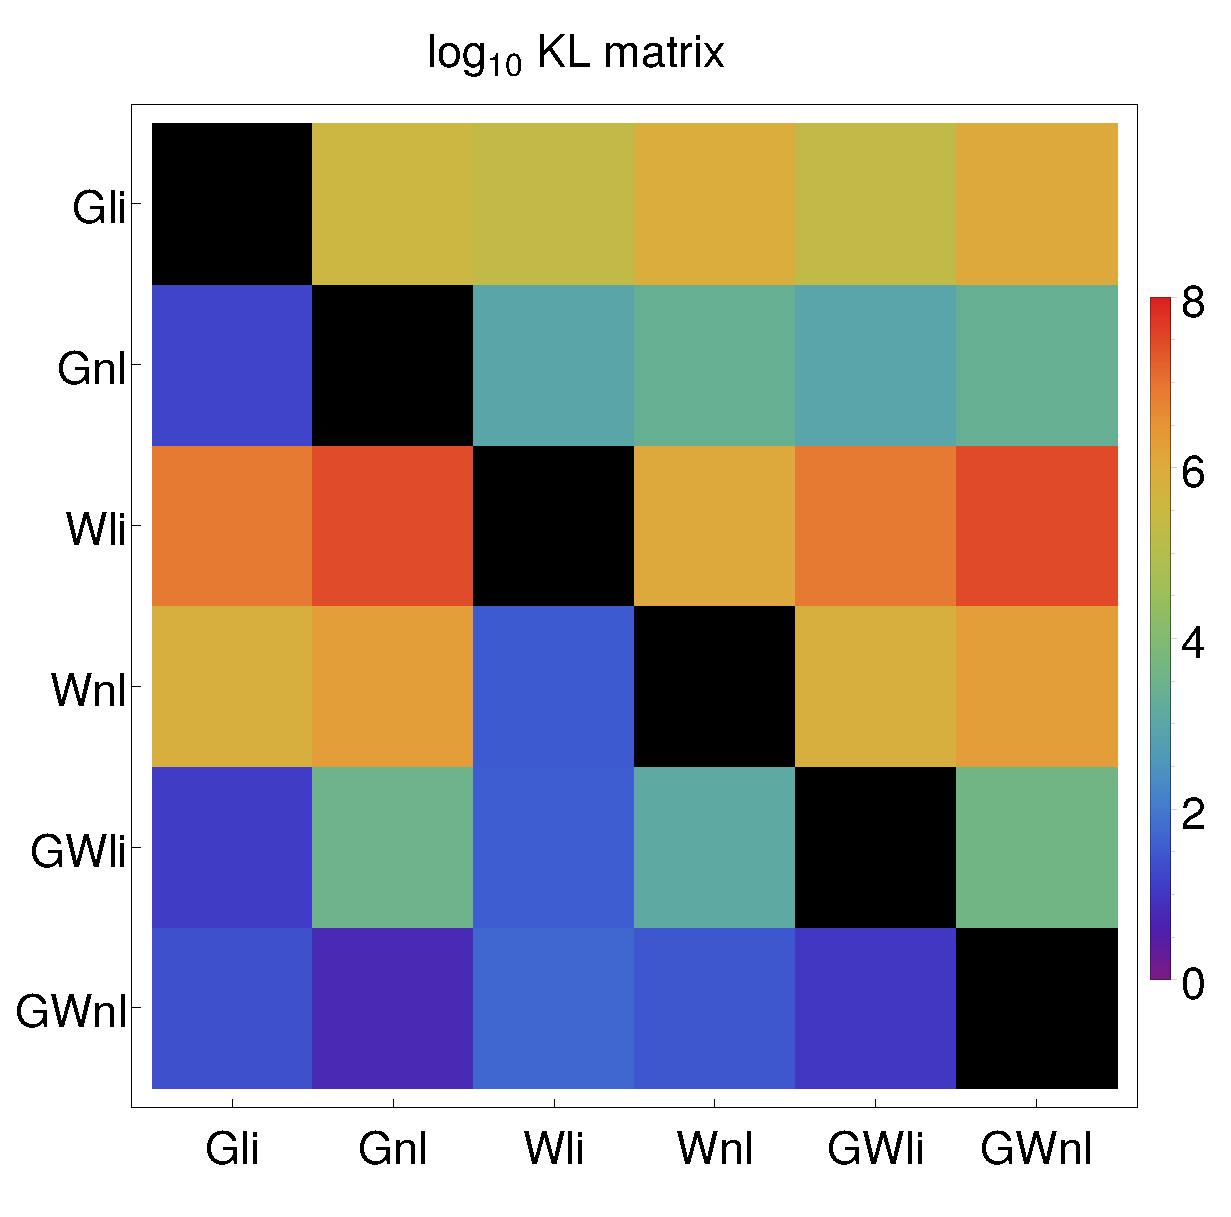
\includegraphics[width=0.45\linewidth]{Chapters/linear-nonlinear-MG-forecasts/figures/KL-divergence/KL-Matrix-all-obs-noPlanck-new}
	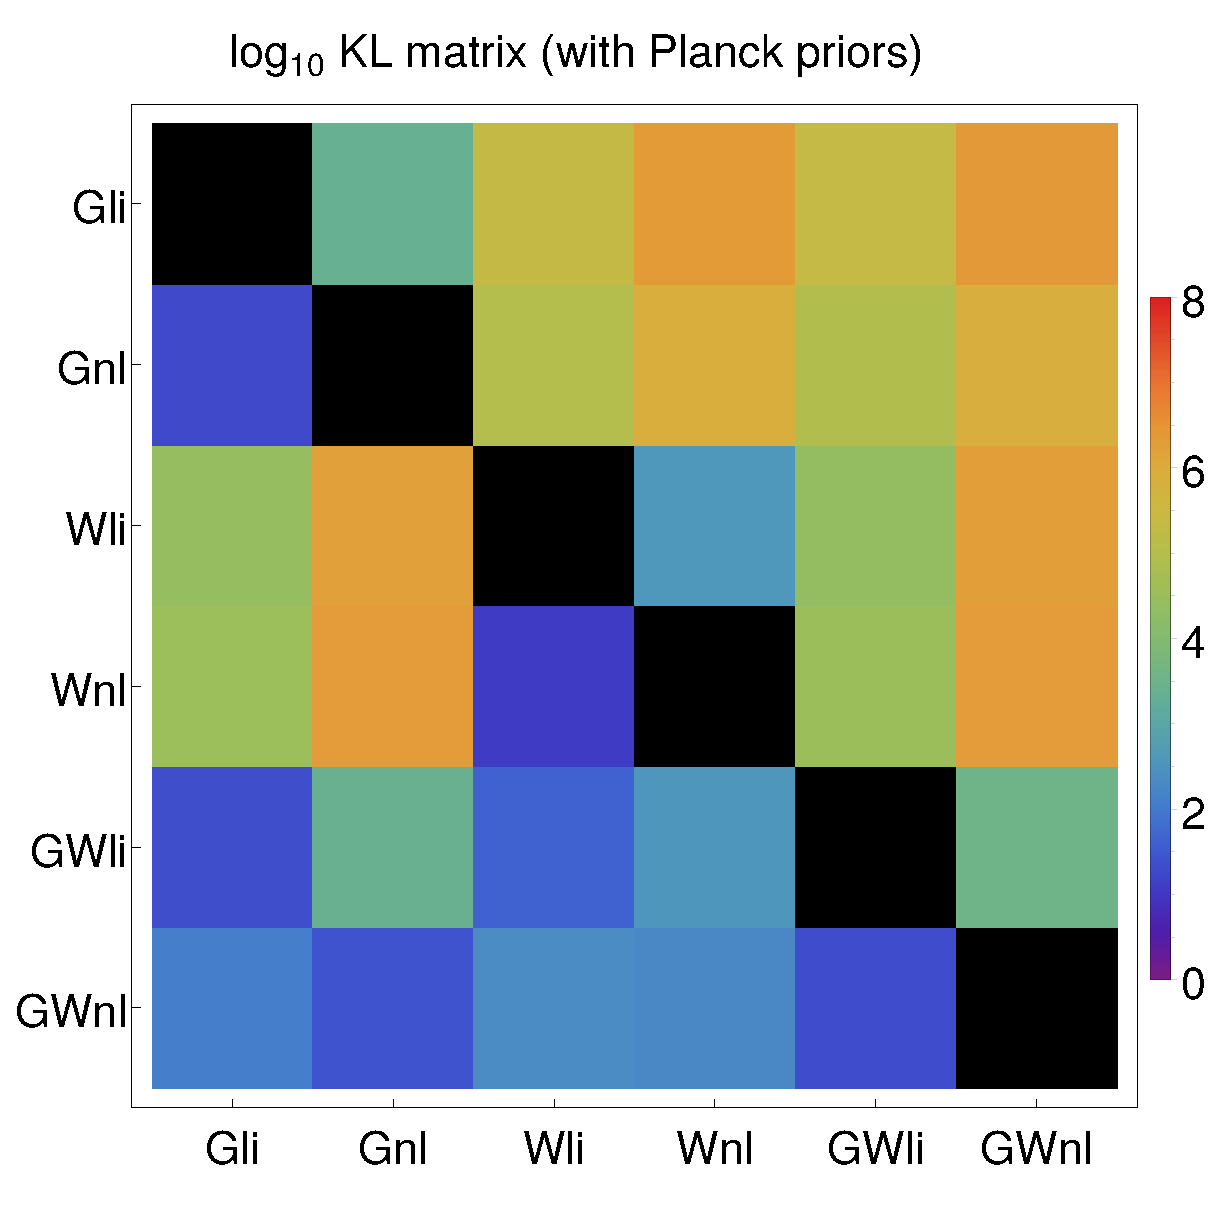
\includegraphics[width=0.45\linewidth]{Chapters/linear-nonlinear-MG-forecasts/figures/KL-divergence/KL-Matrix-all-obs-withPlanck-new}
	\caption[Kullback-Leibler divergence matrices for Euclid forecasts.]{Kullback-Leibler divergence matrices $\mathcal{K}_{ij}$. This matrix represents graphically
		the information gain between all possible observables in the redshift
		binned parameterization of section \ref{sec:Results:-Redshift-Binned}. 
		We have plotted here the logarithm of the KL-divergence matrix, for illustrative purposes. 
		Therefore the diagonal is $-\infty$ and it is represented by a black color. 
		\textbf{Left:} KL matrix without \planck\ priors. 
		The maximum gain is about $10^7$ when going from WL(lin) to GC+WL(non-linear) 
		and we can observe that GC+WL does not gain extra information when complemented with the other observables, which is expected.
		\textbf{Right:} In this case we compare the observables, when a \planck\ prior is added beforehand. 
		The overall information gain is now smaller, with a maximum of about $10^6$. 
		The maximum gain comes when comparing WL (linear and non-linear) to GC and GC+WL (non-linear). 
	}
	\label{fig:kl-matrices}
\end{figure}



\subsection{CMB \planck\ priors}
\label{sub:Fisher-Planck}
Alongside the information brought by LSS probes,
we also include CMB priors on the parameterizations considered. In
order to obtain these, we analyze the binned and parameterized approaches
described in Section \ref{sec:Parameterizing-Modified-Gravity} with
the {\it Planck}+BSH combination of CMB and background (BAO+SN-Ia+$H_{0}$)
datasets discussed in the \planck\ Dark Energy and Modified Gravity paper
\cite{planck_collaboration_planck_2016}.
We use a Markov Chain Monte Carlo (MCMC) approach, using the publicly
available code \texttt{COSMOMC} \cite{lewis_cosmological_2002,lewis_efficient_2013},
interfaced with our modified version of \texttt{MGCAMB}. The MCMC
chains sample the parameter vector $\Theta$ which contains the standard
cosmological parameters
$\{\omega_{b}\equiv\Omega_{b}h^{2},\,\omega_{c}\equiv\Omega_{c}h^{2},\,\theta_{\rm MC},\,\tau,n_{s},\ln{10^{10}A_{s}}\}$
to which we add the $E_{ij}$ parameters when we parameterize the time
evolution of $\mu$ and $\eta$ with continuous functions of the scale factor, 
and the $\mu_{i},\ \eta_{i}$ parameters in the binned
case. On top of these, also the 17 nuisance parameters of the \planck\
analysis are included. From the MCMC analysis of the \planck\ likelihood
we obtain a covariance matrix in terms of the parameters $\Theta$.
We marginalize over the nuisance parameters and over the optical
depth $\tau$ since this parameter does not enter into
the physics of large scale structure formation.

$\theta$ is usually the ratio of sound horizon
to the angular diameter distance at the time of decoupling. Since
calculating the decoupling time $z_{\rm CMB}$ is relatively time consuming,
as it involves the minimization of the optical transfer function,
\texttt{COSMOMC} uses instead an approximate quantity $\theta_{\rm MC}$
based on the following fitting formula from \cite{hu_small_1996}
\begin{align}
z_{\rm CMB} & =1048\times(1+0.00124\omega_{b}^{-0.738})\nonumber \\
 &
\times\left(1+0.0783\omega_{b}^{-0.238}/(1+39.5\omega_{b}^{0.763})\right.\nonumber
\\
 & \times\left.(\omega_{d}+\omega_{b})^{0.560/(1+21.1\omega_{b}^{1.81})}\right)
\end{align}
where $\omega_{d}\equiv(\Omega_{c}+\Omega_{\nu})h^{2}$.
The sound horizon is defined as 
\begin{equation}
r_{s}(z_{\rm CMB})=cH_{0}^{-1}\int_{z_{\rm CMB}}^{\infty}\mbox{d}z\frac{c_{s}}{E(z)}
\end{equation}
where the sound speed is $c_{s}=1/\sqrt{3(1+\overline{R}_{b}a)}$with
the baryon-radiation ratio being $\overline{R}_{b}a=3\rho_{b}/4\rho_{\gamma}$.
$\overline{R}_{b}=31500\Omega_{b}h^{2}(T_{\rm CMB}/2.7\mbox{K})^{-4}$.
However, \texttt{CAMB }approximates it as
$\overline{R}_{b}a=30000a\Omega_{b}h^{2}$.

Therefore we first marginalize the covariance matrix over the nuisance
parameters and the parameter $\tau$, which cannot be constrained
by LSS observations. Then, we invert the resulting matrix, to obtain a \planck\
prior Fisher matrix and then use a Jacobian to convert between the
MCMC parameter basis $\Theta_{i}$ and the GC-WL parameter basis $\theta_{i}$.
We use the formulas above for the sound horizon $r_{s}$ and the angular
diameter distance $d_{A}$ to calculate the derivatives of $\theta_{\rm MC}$
with respect to the parameters of interest. Our Jacobian is then simply (see Appendix \ref{sec:appjac} for details)
\begin{equation}
J_{ij}=\frac{\partial\Theta_{i}}{\partial\theta_{j}} \, .
\end{equation}

\subsection{Systematic bias on cosmological parameters}

In this section we will quantify the effect of the systematic errors
due to the uncertainties on the non-linear power spectrum. We will
show how big this systematic bias would be, if we used for our forecasts
a power spectrum which is not the ``correct'' one, for example one
obtained from a single N-body realization. For the following discussion
on systematic biases, we will use the expressions derived in the Appendix
B of \cite{taylor_probing_2007}.

The linear bias on a cosmological parameter $\delta\theta_{i}$ due
to the bias $\delta\psi_{i}$ in a parameter of the model which we
assume fixed and cannot be measured is given by: 

\begin{equation}
\delta\theta_{i}=-\left[F^{\theta\theta}\right]_{ik}^{-1}F_{kj}^{\theta\psi}\delta\psi_{j}\label{eq:syst.bias}
\end{equation}


In our case we will have only one systematic parameter $\psi$, which
controls the difference between the ``true'' power spectrum $P_{true}$
and and our simulated power spectrum $P_{num}$:

\[
P_{\psi}=\psi P_{num}+(1-\psi)P_{true}
\]
$\psi$ can vary continously so that for $\psi=1$ we recover $P_{num}$,
while for $\psi=0$ we obtain $P_{true}$. We can define 
the relative difference between $P_{true}$ and $P_{num}$ as:
\begin{equation}
\sigma_{p}(k,z)\equiv\frac{P_{num}(k,z)-P_{true}(k,z)}{P_{true}(k,z)}
\end{equation}


The $F^{\theta\theta}$ in eqn.\ref{eq:syst.bias} above is simply
the usual Fisher matrix: 
\[
F^{\theta\theta}=\frac{1}{2}\mbox{tr}\left(C^{-1}\partial_{i}^{\theta}CC^{-1}\partial_{j}^{\theta}C\right)
\]
while the pseudo-Fisher matrix between measured and assumed parameters
$F^{\theta\psi}$ is:

\begin{equation}
F_{ij}^{\theta\psi}=\frac{1}{2}\mbox{tr}\left(C^{-1}\partial_{i}^{\theta}CC^{-1}\partial_{j}^{\psi}C\right)
\end{equation}
which for one systematic parameter only, is just a column vector.

In the case of galaxy Clustering we will compute $F^{\theta\psi}$
in the following way, using the fact that for $\psi=1$, $C=P_{num}(k,z)+n^{-1}(z)$
and $P_{\psi}|_{\psi=1}=P_{num}$:

\begin{equation}
F_{i}^{\theta\psi}\propto\int\mbox{d}k\, k^{2}\left(\frac{n_{eff}(z)P_{num}(k,z)}{n_{eff}(z)P_{num}(k,z)+1}\right)^{2}\left(\frac{1}{P_{num}(k,z)}\right)^{2}\left.\frac{\partial P_{\psi}}{\partial\psi}\right|_{\psi=1}\frac{\partial P_{num}}{\partial\theta_{i}}\label{eq:pseudo-Fisher}
\end{equation}


in this step we have assumed that we have no systematic parameters
affecting the galaxy number density $n(z)$ and therefore, its derivative
w.r.t $\psi$ vanishes. Also, for notational simplicity we left out the integral over $\mu$ and the
form of the observed power spectrum.

We have then $\partial_{\psi}P_{\psi}=-P_{true}+P_{num}=P_{true}\sigma_{p}(k,z)$
and we just need to perform eqn. \ref{eq:pseudo-Fisher} with eqn.
\ref{eq:syst.bias} in order to obtain the systematic biases on the
cosmological parameters.

In the following table \ref{tab:systbias} we present the results
on the systematic bias, for a standard $\lcdm$ forecast, for different
maximum $k$ coverages, up to a maximum $k$ of $1.1$h/Mpc. We will
regard as a ``true'' power spectrum $P_{true}$, the one obtained
by the Cosmic (Franken) Emulator \cite{heitmann_coyote_2014}, since
they have performed a careful analysis of resolution effects using
a large set of simulations and claim to be accurate for $k<1.0\,\mbox{h/Mpc}$
at the 1\% percent level compared to state of the art N-body simulations.
On the other hand, the numerical ``biased'' power spectrum $P_{num}$,
is the one obtained from the CoDECS $\lcdm$ run, which consists on
only one realization. We have left out the CDE coupling parameter
$\beta$, since in that case we do not have any other prediction in
the non-linear regime to compare with. 



The results of table \ref{tab:systbias} show how important it is
to model accurately the non-linear power spectrum in order to make
forecasts and to analyze the upcoming data of large scale structure
surveys like Euclid \cite{amendola_cosmology_2012-short}. The systematic
errors on the cosmological parameters can be bigger than the statistical
errors (compare to table \ref{tab:1-sigmaerrors-nl-GC-1} and figure
\ref{fig:kmax-change-lin-nonlin} in the results section below). This
is the case if, as in our example scenario, we would use a non-linear
power spectrum that is inaccurate by about 10-15\% in the non-linear
regime at higher redshifts (which was shown in figure \ref{fig:Error-comp-Halofit-CosmicEmu}).
Therefore, it is well justified to choose for our Fisher forecasts
the Cosmic Emulator as the ``true'' $\lcdm$ non-linear power spectrum
estimator, since this is the most accurate predictor up to date. It
would still be interesting to know how robust is the signal of the
coupling parameter $\beta$ with respect to changes in the other parameters
or in the $\lcdm$ non-linear prediction, but as long as we do not
have better and faster semianalytic methods applicable to general
models of dark energy, the estimation of systematic biases of extra
parameters is an impossible task.

\section{The equations and structure of the \textsc{FisherTools} code \label{sec:FisherTools-code}}
\begin{itemize}
\item This serves as a manual for the Fisher Tools code.
\end{itemize}

If one wishes to place constraints on the normalization of the power
spectrum, $\sigma_{8}$, then $P(k,z)$ can be written as:

\begin{equation}
P(k,z)=\sigma_{8}^{2}\tilde{P}(k,z)\label{eq:normalizedPk}
\end{equation}
where $\tilde{P}(k,z)$ is the normalized power spectrum. The normalization
$s_{R}$of the power spectrum (which is equivalent to the variance
smoothed over a scale $R$) is given by:
\begin{equation}
s_{R}=\frac{1}{2\pi^{2}}\int_{k_{min}}^{k_{max}}k^{2}P(k,z=0)W_{R}^{2}(kR)\label{eq:normalizationPk}
\end{equation}


The window function smooths $P(k,z)$ over the scale $R$ and has
the form: $W(x)=3(\sin(x)-x\cos(x))/x^{3}$, where $x$ is a dimensionless
variable. This term comes from assuming spherical symmetry and performing
the angle integration of the 3-D power spectrum $P(\vec{k})$. If
one chooses $R=8\mbox{h}^{-1}\mbox{Mpc}$ and $[k]=\mbox{h}/\mbox{Mpc}$,
then we recover the usual $s_{R}=\sigma_{8}^{2}$. The normalization
$\sigma_{8}$ is a quantity defined only in linear theory, which means
that in Eqn. \ref{eq:normalizationPk} either $P(k,z)$ is linear
or the integration limits are chosen in such a way that only the linear
normalization is taken into account, so that usually one should take
$k_{max}\approx0.1$. The normalized power spectrum is simply: 
\begin{equation}
\tilde{P}(k,z)=\frac{1}{s_{R}}P(k,z)
\end{equation}


Due to the of the fact that $\sigma_{8}$ is a linear quantity, we
can use it as an independent cosmological parameter, because we can
rescale it arbitrarily before it is compared with observations. It
is then completely degenerate with the initial primordial amplitude
of the power spectrum, $\mathcal{A}_{s}$, and one can replace one
parameter by the other, fixing just one of both.\footnote{One has to emphasize that this can only be done for linear power spectra,
	because if one takes nonlinear density fluctuations into account for
	calculating a non-linear $P(k,z)$, a different primordial amplitude
	of fluctuations has a non-linear effect at small scales in the so
	called ``non-linear bump''. The degeneracy between $\mathcal{A}_{s}$
	and $\sigma_{8}$ is then broken.}

Furthermore if one wishes to express a linear power spectrum $P(k,z)$
in terms of the primordial power spectrum, the growth $G(z)$ and
the transfer functions $T(k)$, one can write Eqn. \ref{eq:normalizedPk}
as: 
\begin{equation}
P(k,z)=\frac{\sigma_{8}^{2}}{s_{R}}G^{2}(z)T^{2}(k)k^{ns}\mathcal{A}_{s}
\end{equation}
being careful to take either $\sigma_{8}$ or $\mathcal{A}_{s}$ as
a primordial parameter and not both. In the case in which $\mathcal{A}_{s}$
is the cosmological parameter, the ratio $\frac{\sigma_{8}^{2}}{s_{R}}$
should be 1. The growth function $G(z)$ depends on the cosmological
parameters $\theta_{i}$ and is defined to be normalized to unity
today: $G(z=0)=1$. The quantity $\sigma_{8}^{2}G^{2}(z)\equiv\sigma_{8}(z)$
can be defined accordingly and can be used as an independent and time-dependent
cosmological parameter too. 


When we perform the numerical derivatives
of $P_{obs}(k,\mu,z)$, we have to take into account that not only
the power spectrum and the background functions change, when the cosmological
parameters are modified, but also $\mu$ and $k$ are changed by a
geometrical factor depending on $H(z)$ and $D_{A}(z)$, due to the
Alcock-Paczinsky effect \citep{alcock1979anevolution}.

\subsubsection{Derivatives of the observed power spectrum}

For the calculation of the Fisher matrix, one needs to take derivatives
of the logarithm of the observed power spectrum $P_{obs}(k,z,\mu)$
at the central value $\bar{z}$ of each redshift bin. (see equation
for the Fisher matrix). There are two options here in terms of the
practical and numerical approach: 
\begin{itemize}
	\item One calculates numerically: 
	\begin{equation}
	\left.\frac{\mbox{d}\ln P_{{\rm obs}}\left(\bar{z},k,\mu;\theta_{i}\right)}{\mbox{d}\theta_{i}}\right|_{fid}=\frac{P_{{\rm obs}}\left(\bar{z},k,\mu;\theta_{i}^{+}\right)-P_{{\rm obs}}\left(\bar{z},k,\mu;\theta_{i}^{-}\right)}{2\varepsilon\theta_{i}^{fid}\times P_{{\rm obs}}\left(\bar{z},k,\mu;\theta_{i}^{fid}\right)}
	\end{equation}
	where $\theta_{i}^{+}$, $\theta_{i}^{-}$ represent the parameter
	$\theta_{i}$ evaluated at $\pm\varepsilon$ around the fiducial value
	$\theta_{i}^{fid}$:
	\begin{equation}
	\theta_{i}^{\pm}=\theta_{i}^{fid}(1\pm\varepsilon)
	\end{equation}
	However this assumes that all functions inside $P_{{\rm obs}}(\bar{z},k,\mu;\theta_{i})$
	can be evaluated at $\theta_{i}^{\pm}$. Since this is not the case
	for the bias $b(z)$, one needs to add a further intermediate variable
	(see section \ref{sec:Marginalization} below on marginalization).
	\item One uses intermediate variables, namely the functions in Eqn. \ref{eq:obs-power-basic},
	which depend on $\theta_{i}$, and with the help of the chain rule
	one can write:
	\begin{align}
	\left.\frac{\mbox{d}\ln P_{{\rm obs}}\left(\bar{z},k,\mu;\theta_{i}\right)}{\mbox{d}\theta_{i}}\right|_{fid} & =\frac{\partial\ln P_{obs}\left(\bar{z},k,\mu;\theta_{i}\right)}{\partial\ln P_{s}(\bar{z})}\frac{\partial\ln P_{s}(\bar{z})}{\partial\theta_{i}}+\frac{\partial\ln P_{obs}\left(\bar{z},k,\mu;\theta_{i}\right)}{\partial\ln f(\bar{z})}\frac{\partial\ln f(\bar{z})}{\partial\theta_{i}}\nonumber \\
	& +\frac{\partial\ln P_{obs}\left(\bar{z},k,\mu;\theta_{i}\right)}{\partial\ln H(\bar{z})}\frac{\partial\ln H(\bar{z})}{\partial\theta_{i}}+\frac{\partial\ln P_{obs}\left(\bar{z},k,\mu;\theta_{i}\right)}{\partial\ln D_{A}(\bar{z})}\frac{\partial\ln D_{A}(\bar{z})}{\partial\theta_{i}}\nonumber \\
	& +\frac{\partial\ln P_{obs}\left(\bar{z},k,\mu;\theta_{i}\right)}{\partial\ln P(k,\bar{z})}\frac{\partial\ln P(k,\bar{z})}{\partial\theta_{i}}+\frac{\partial\ln P_{obs}\left(\bar{z},k,\mu;\theta_{i}\right)}{\partial\ln b(\bar{z})}\frac{\partial\ln b(\bar{z})}{\partial\theta_{i}}\label{eq:derivatives-of-lnPobs}\\
	& +{\color{red}\frac{\partial\ln P_{obs}\left(\bar{z},k,\mu;\theta_{i}\right)}{\partial k}\frac{\partial k}{\partial\theta_{i}}+\frac{\partial\ln P_{obs}\left(\bar{z},k,\mu;\theta_{i}\right)}{\partial\mu}\frac{\partial\mu}{\partial\theta_{i}}}\nonumber 
	\end{align}
	where we have ignored the dependence on the damping terms of Eqn.
	\ref{eq:obs-power-basic} for simplicity. The last two terms are non-vanishing
	if one takes the Alcock-Paczynski effect into account for $k$ and
	$\mu$, since they are affected by geometrical terms also (see AP-effect
	section \ref{sub:The-Alcock-Paczynski-Effect} below).
\end{itemize}
One then has to calculate the intermediate derivatives of $\ln P_{obs}(z,k,\mu;\theta_{i})$
with respect to $P_{s}$, $D_{A}$, $H$, $f$ and $b$ using Eqn.
\ref{eq:obs-power-basic}. The logarithm of these quantities is used,
because it simplifies considerably the equations. Notice that the
growth $G(z)$ is inside the definition of $P(k,z)$ so it is not
needed as an intermediate variable, however it can be also used if
wanted. It is important to stress here that the derivatives are calculated
at the \emph{fiducial} value of the parameters, including the fiducial
values of the cosmological functions. The fiducial value of the shot
noise is zero, $P_{s}^{fid}(z)=0$. And under this choice the derivatives
are:

\begin{subequations}
	
	\begin{align}
	\frac{\partial\ln P_{obs}\left(\bar{z},k,\mu;\theta_{i}\right)}{\partial\ln P_{s}(\bar{z})} & =\frac{1}{P_{obs}\left(\bar{z},k,\mu;\theta_{i}\right)}\\
	\frac{\partial\ln P_{obs}\left(\bar{z},k,\mu;\theta_{i}\right)}{\partial\ln f(\bar{z})} & =\frac{2\beta(\bar{z})\mu^{2}}{1+\beta(\bar{z})\mu^{2}}\\
	\frac{\partial\ln P_{obs}\left(\bar{z},k,\mu;\theta_{i}\right)}{\partial\ln b(\bar{z})} & =\frac{2}{1+\beta(\bar{z})\mu^{2}}\\
	\frac{\partial\ln P_{obs}\left(\bar{z},k,\mu;\theta_{i}\right)}{\partial\ln H(\bar{z})} & =1\\
	\frac{\partial\ln P_{obs}\left(\bar{z},k,\mu;\theta_{i}\right)}{\partial\ln D_{A}(\bar{z})} & =-2\\
	\frac{\partial\ln P_{obs}\left(\bar{z},k,\mu;\theta_{i}\right)}{\partial\ln P(k,\bar{z})} & =1
	\end{align}
	\label{eq: partial-derivs-subeqns}
	
\end{subequations}

If for the moment and for simplicity we neglect the extra shot noise
contribution $P_{s}$ and the dependence of $k$ and $\mu$ on the
change of cosmological parameters (see AP-effect section below) we
get for each derivative of $P_{obs}(k,\mu,z)$with respect to a cosmological
parameter $\theta_{i}$:

\begin{align}
\left.\frac{\mbox{d}\ln P_{{\rm obs}}\left(\bar{z},k,\mu;\theta_{i}\right)}{\mbox{d}\theta_{i}}\right|_{fid} & =\frac{\partial\ln P(k,\bar{z})}{\partial\theta_{i}}+\frac{\partial\ln H(\bar{z})}{\partial\theta_{i}}-2\frac{\partial\ln D_{A}(\bar{z})}{\partial\theta_{i}}\nonumber \\
& +\frac{2\beta(\bar{z})\mu^{2}}{1+\beta(\bar{z})\mu^{2}}\frac{\partial\ln f(\bar{z})}{\partial\theta_{i}}+\frac{2}{1+\beta(\bar{z})\mu^{2}}\frac{\partial\ln b(\bar{z})}{\partial\theta_{i}}\label{eq:derivatives-of-lnPobs-simplified-1}
\end{align}


We see that by using intermediate variables, the space of parameters
to be evaluated for the Fisher matrix has been extended by 4 new terms
(they could be more if $P_{obs}$ depends on further cosmological
functions): 

\begin{equation}
\zeta=\{1,1,-2,\frac{2\beta(\bar{z})\mu^{2}}{1+\beta(\bar{z})\mu^{2}},\frac{2}{1+\beta(\bar{z})\mu^{2}}\}\label{eq:dPobsDFuncts}
\end{equation}


The new ``vector'' of derivatives has the form:

\begin{equation}
\Theta=\{\frac{\partial\ln P(k,\bar{z})}{\partial\theta_{i}},1,-2,\frac{2\beta(\bar{z})\mu^{2}}{1+\beta(\bar{z})\mu^{2}},\frac{2}{1+\beta(\bar{z})\mu^{2}}\}\label{eq:bigThetaVector}
\end{equation}
notice that $\theta_{i}$ is a vector also, so that this vector has
a number of components equal to: $\dim(\Theta)=\dim(\theta)+4$.

Since the Fisher matrix is a tensor product of a vector of derivatives,
we can express it as:
\begin{equation}
F_{ij}\approx\frac{\mbox{d}\ln P_{{\rm obs}}}{\mbox{d}\theta_{i}}\frac{\mbox{d}\ln P_{{\rm obs}}}{\mbox{d}\theta_{j}}\approx(\Theta\otimes\Theta)_{ij}\label{eq:FisherTensorProd-1}
\end{equation}


However this is only valid at one single redshift bin and if one wants
to add together Fisher matrices at different redshift bins, one has
to take into account that each $D_{A}(\bar{z}_{i})$, $H(\bar{z}_{i})$,
$f(\bar{z}_{i})$ and $b(\bar{z}_{i})$ is an independent parameter
but we will come to that later. 


\subsubsection{Projecting back to the fundamental cosmological parameters}

If one wishes to express the Fisher matrix just in terms of fundamental
cosmological parameters again, then one needs to perform the variable
transformation back using a so-called Jacobian. This can be seen more
clearly if one expresses Eqns. \ref{eq:derivatives-of-lnPobs}, \ref{eq: partial-derivs-subeqns}
and \ref{eq:derivatives-of-lnPobs-simplified-1} as:

\begin{equation}
\frac{\mbox{d}\ln P_{obs}(\mathbf{T}(\boldsymbol{\theta}))}{\mbox{d}\boldsymbol{\theta}_{i}}=\frac{\partial\ln P_{obs}}{\partial\mathbf{T}{}_{j}}\frac{\partial\mathbf{T}_{j}}{\partial\boldsymbol{\theta}_{i}}
\end{equation}
where $\mathbf{T}_{i}=\{\ln P,\,\ln H,\,\ln D_{A},\,\ln f,\,\ln b\}$
and $\partial P_{obs}/\partial\mathbf{T}{}_{i}=\zeta$ from Eqn. \ref{eq:dPobsDFuncts}.
The Jacobian is then simply: 

\begin{equation}
J=\frac{\partial\mathbf{T}_{j}}{\partial\boldsymbol{\theta}_{i}}\label{eq:jacobian}
\end{equation}


The Fisher matrix 

\begin{equation}
\tilde{F}_{ab}\approx(\zeta\otimes\zeta)_{ab}\approx\frac{\partial\ln P_{obs}}{\partial\mathbf{T}{}_{a}}\frac{\partial\ln P_{obs}}{\partial\mathbf{T}{}_{b}}
\end{equation}
formed in the intermediate variables $\boldsymbol{T}$ can be transformed
to the usual one $F$ by calculating:

\begin{equation}
F_{ab}\approx\frac{\mbox{d}\ln P_{obs}}{\mbox{d}\boldsymbol{\theta}{}_{a}}\frac{\mbox{d}\ln P_{obs}}{\mbox{d}\boldsymbol{\theta}{}_{b}}\approx\frac{\partial\ln P_{obs}}{\partial\mathbf{T}{}_{j}}\frac{\partial\mathbf{T}_{j}}{\partial\boldsymbol{\theta}_{a}}\frac{\partial\ln P_{obs}}{\partial\mathbf{T}{}_{j}}\frac{\partial\mathbf{T}_{j}}{\partial\boldsymbol{\theta}_{b}}=J^{T}\,\tilde{F}\,J
\end{equation}


In the praxis however, for calculating the full Fisher matrix, one
interchanges the first element of $\zeta$ by the first element $\partial\boldsymbol{F}_{1}/\partial\boldsymbol{\theta}_{i}$
(corresponding to the derivatives of the power spectrum $P(k,z)$)
since one needs to integrate values in $k$ and $z$. That is why
one uses the vector $\Theta$ from Eqn. \ref{eq:bigThetaVector}.
In this case the Jacobian and the $\tilde{F}$ do not look like the
ones presented above. This is however, mathematically equivalent at
this point.


\subsubsection{The Alcock-Paczynski Effect\label{sub:The-Alcock-Paczynski-Effect}}

The Alcock-Paczynski effect (AP) relies on the fact that the scales
$k$ and the direction cosines $\mu$ are changed by geometrical factors
of distance, when the cosmological parameters are changed. This means
that $k$ and $\mu$ depend on $H(z)$ and $D_{A}(z)$ and therefore
are also indirectly functions of the cosmological parameters $\theta_{i}$.
The AP formulas relating the fiducial values of $k_{fid}$ and $\mu_{fid}$
to their transformed values are:

\begin{align}
k_{AP} & =R_{AP}(\mu;\theta)k_{fid}\\
\mu_{AP} & =\frac{H(z;\theta)}{H(z;\theta_{fid})}\frac{\mu_{fid}}{R_{AP}(\mu;\theta)}
\end{align}
where the geometrical function $R_{AP}$ is defined as:

\begin{equation}
R_{AP}(\mu;\theta)=\sqrt{\frac{[D_{A}(z;\theta)H(z;\theta)\mu_{fid}]^{2}-[(D_{A}(z;\theta_{fid})H(z;\theta_{fid})]^{2}(\mu_{fid}-1)}{[D_{A}(z;\theta)H(z;\theta_{fid})]^{2}}}
\end{equation}


The last two terms of Eqn. \ref{eq:derivatives-of-lnPobs} come from
the fact that now $k=k(H(z;\theta),D_{A}(z;\theta))$ and $\mu=k(H(z;\theta),D_{A}(z;\theta))$,
so that one has to use the chain rule for the derivative of $P_{obs}(k,\mu,z;\theta)$:

\begin{align}
\frac{\partial\ln P_{obs}\left(\bar{z},k,\mu;H(z);\theta_{i}\right)}{\partial\ln H(z)} & =\frac{\partial\ln P_{obs}\left(\bar{z},k,\mu;\theta_{i}\right)}{\partial\ln H(z)}\\
& +\frac{\partial\ln P_{obs}\left(\bar{z},k,\mu;\theta_{i}\right)}{\partial\mu}\frac{\partial\mu}{\partial\ln H(z)}+\frac{\partial\ln P_{obs}\left(\bar{z},k,\mu;\theta_{i}\right)}{\partial k}\frac{\partial k}{\partial\ln H(z)}\nonumber 
\end{align}
and similarly for the dependence on $D_{A}(z)$.

Now we can write down explicitly the intermediate derivatives (evaluated
at the fiducial value as usual):

\begin{equation}
\frac{\partial\ln P_{obs}\left(\bar{z},k,\mu;\theta_{i}\right)}{\partial k}=\frac{\partial\ln P\left(\bar{z},k;\theta_{i}\right)}{\partial k}
\end{equation}


\begin{equation}
\frac{\partial\ln P_{obs}\left(\bar{z},k,\mu;\theta_{i}\right)}{\partial\mu}=\frac{4\beta(z)\mu}{1+\beta(z)\mu^{2}}
\end{equation}
and the derivatives of $k$ and $\mu$ with respect to $\ln D_{A}$
and $\ln H$ are:

\begin{subequations}
	
	\begin{align}
	\frac{\partial\mu}{\partial\ln D_{A}(z)} & =-\mu(\mu^{2}-1)\\
	\frac{\partial\mu}{\partial\ln H(z)} & =-\mu(\mu^{2}-1)\\
	\frac{\partial k}{\partial\ln D_{A}(z)} & =k(\mu^{2}-1)\\
	\frac{\partial k}{\partial\ln H(z)} & =k\mu^{2}
	\end{align}
	
	
	\label{eq: derivs-of-k-mu-AP}\end{subequations}

The interesting thing about Eqns.\ref{eq: derivs-of-k-mu-AP} is that
one can see that when evaluating the derivative of $P_{obs}$ w.r.t
a cosmological parameter, the scales $k$ and the direction cosine
angles $\mu$ get mixed, giving a very powerful probe of cosmology.
Using this, the vectors that form the Fisher matrix (either $\zeta$
or $\Theta$, depending on the choice) have to be extended in their
indices corresponding to $\ln D_{A}$ and $\ln H$. So that they are
now more complicated:

\begin{multline}
\Theta=\left\{ \frac{\partial\ln P(k,\bar{z})}{\partial\theta_{i}},1+\frac{4\beta(z)\mu}{1+\beta(z)\mu^{2}}(-\mu(\mu^{2}-1))+\frac{\partial\ln P\left(\bar{z},k;\theta_{i}\right)}{\partial k}k\mu^{2},\right.\\
\left.-2+\frac{4\beta(z)\mu}{1+\beta(z)\mu^{2}}(-\mu(\mu^{2}-1))+\frac{\partial\ln P\left(\bar{z},k;\theta_{i}\right)}{\partial k}k(\mu^{2}-1),\frac{2\beta(\bar{z})\mu^{2}}{1+\beta(\bar{z})\mu^{2}},\frac{2}{1+\beta(\bar{z})\mu^{2}}\right\} 
\end{multline}


However, using the procedure described above, one can see that the
Fisher matrix will have the same dimensions and that the Jacobian
will be the same as in Eqn. \ref{eq:jacobian}.


%\subsection{Marginalization\label{sec:Marginalization}}
%
%When using the form of the observed power spectrum presented before,
%it is not always possible to ``project back'' the matrix $\tilde{F}$
%into the matrix $F$ which contains only fundamental cosmological
%parameters. This is the case for the bias or the extra shot noise,
%since there we do not know how the derivatives $\partial\ln b(z)/\partial\theta_{i}$
%or $\partial P_{s}(z)/\partial\theta_{i}$ look like, since those
%are observational and/or phenomenological quantities which do not
%yet have a model in terms of fundamental cosmological parameters.
%Therefore, these terms will always remain and cannot be expressed
%as a function of cosmological parameters and have to be either fixed
%or marginalized over. In terms of the Fisher matrix $F_{ij}$, the
%marginalization is performed easily by removing from the inverse $F_{ij}^{-1}$
%all rows and columns corresponding to the index of the quantity to
%marginalize. More about this will be explained later on.



\subsection{Validation of the code within the Euclid collaboration}
\begin{itemize}
\item 4 Steps: from the basics to the more complicated
\item Shape parameters, z-obswevables and non-diagonal terms
\item WL: Cases
\end{itemize}

\subsection{Extensions of the Fisher matrix approach to higher orders}
\begin{itemize}
\item Taylor expansion of the Fisher matrix
\item Fisher tensors
\item Variations in parameter space
\end{itemize}



%----------------------------------------------------------------------------------------